\documentclass[1p]{elsarticle_modified}
%\bibliographystyle{elsarticle-num}

%\usepackage[colorlinks]{hyperref}
%\usepackage{abbrmath_seonhwa} %\Abb, \Ascr, \Acal ,\Abf, \Afrak
\usepackage{amsfonts}
\usepackage{amssymb}
\usepackage{amsmath}
\usepackage{amsthm}
\usepackage{scalefnt}
\usepackage{amsbsy}
\usepackage{kotex}
\usepackage{caption}
\usepackage{subfig}
\usepackage{color}
\usepackage{graphicx}
\usepackage{xcolor} %% white, black, red, green, blue, cyan, magenta, yellow
\usepackage{float}
\usepackage{setspace}
\usepackage{hyperref}

\usepackage{tikz}
\usetikzlibrary{arrows}

\usepackage{multirow}
\usepackage{array} % fixed length table
\usepackage{hhline}

%%%%%%%%%%%%%%%%%%%%%
\makeatletter
\renewcommand*\env@matrix[1][\arraystretch]{%
	\edef\arraystretch{#1}%
	\hskip -\arraycolsep
	\let\@ifnextchar\new@ifnextchar
	\array{*\c@MaxMatrixCols c}}
\makeatother %https://tex.stackexchange.com/questions/14071/how-can-i-increase-the-line-spacing-in-a-matrix
%%%%%%%%%%%%%%%

\usepackage[normalem]{ulem}

\newcommand{\msout}[1]{\ifmmode\text{\sout{\ensuremath{#1}}}\else\sout{#1}\fi}
%SOURCE: \msout is \stkout macro in https://tex.stackexchange.com/questions/20609/strikeout-in-math-mode

\newcommand{\cancel}[1]{
	\ifmmode
	{\color{red}\msout{#1}}
	\else
	{\color{red}\sout{#1}}
	\fi
}

\newcommand{\add}[1]{
	{\color{blue}\uwave{#1}}
}

\newcommand{\replace}[2]{
	\ifmmode
	{\color{red}\msout{#1}}{\color{blue}\uwave{#2}}
	\else
	{\color{red}\sout{#1}}{\color{blue}\uwave{#2}}
	\fi
}

\newcommand{\Sol}{\mathcal{S}} %segment
\newcommand{\D}{D} %diagram
\newcommand{\A}{\mathcal{A}} %arc


%%%%%%%%%%%%%%%%%%%%%%%%%%%%%5 test

\def\sl{\operatorname{\textup{SL}}(2,\Cbb)}
\def\psl{\operatorname{\textup{PSL}}(2,\Cbb)}
\def\quan{\mkern 1mu \triangleright \mkern 1mu}

\theoremstyle{definition}
\newtheorem{thm}{Theorem}[section]
\newtheorem{prop}[thm]{Proposition}
\newtheorem{lem}[thm]{Lemma}
\newtheorem{ques}[thm]{Question}
\newtheorem{cor}[thm]{Corollary}
\newtheorem{defn}[thm]{Definition}
\newtheorem{exam}[thm]{Example}
\newtheorem{rmk}[thm]{Remark}
\newtheorem{alg}[thm]{Algorithm}

\newcommand{\I}{\sqrt{-1}}
\begin{document}

%\begin{frontmatter}
%
%\title{Boundary parabolic representations of knots up to 8 crossings}
%
%%% Group authors per affiliation:
%\author{Yunhi Cho} 
%\address{Department of Mathematics, University of Seoul, Seoul, Korea}
%\ead{yhcho@uos.ac.kr}
%
%
%\author{Seonhwa Kim} %\fnref{s_kim}}
%\address{Center for Geometry and Physics, Institute for Basic Science, Pohang, 37673, Korea}
%\ead{ryeona17@ibs.re.kr}
%
%\author{Hyuk Kim}
%\address{Department of Mathematical Sciences, Seoul National University, Seoul 08826, Korea}
%\ead{hyukkim@snu.ac.kr}
%
%\author{Seokbeom Yoon}
%\address{Department of Mathematical Sciences, Seoul National University, Seoul, 08826,  Korea}
%\ead{sbyoon15@snu.ac.kr}
%
%\begin{abstract}
%We find all boundary parabolic representation of knots up to 8 crossings.
%
%\end{abstract}
%\begin{keyword}
%    \MSC[2010] 57M25 
%\end{keyword}
%
%\end{frontmatter}

%\linenumbers
%\tableofcontents
%
\newcommand\colored[1]{\textcolor{white}{\rule[-0.35ex]{0.8em}{1.4ex}}\kern-0.8em\color{red} #1}%
%\newcommand\colored[1]{\textcolor{white}{ #1}\kern-2.17ex	\textcolor{white}{ #1}\kern-1.81ex	\textcolor{white}{ #1}\kern-2.15ex\color{red}#1	}

{\Large $\underline{12a_{1176}~(K12a_{1176})}$}

\setlength{\tabcolsep}{10pt}
\renewcommand{\arraystretch}{1.6}
\vspace{1cm}\begin{tabular}{m{100pt}>{\centering\arraybackslash}m{274pt}}
\multirow{5}{120pt}{
	\centering
	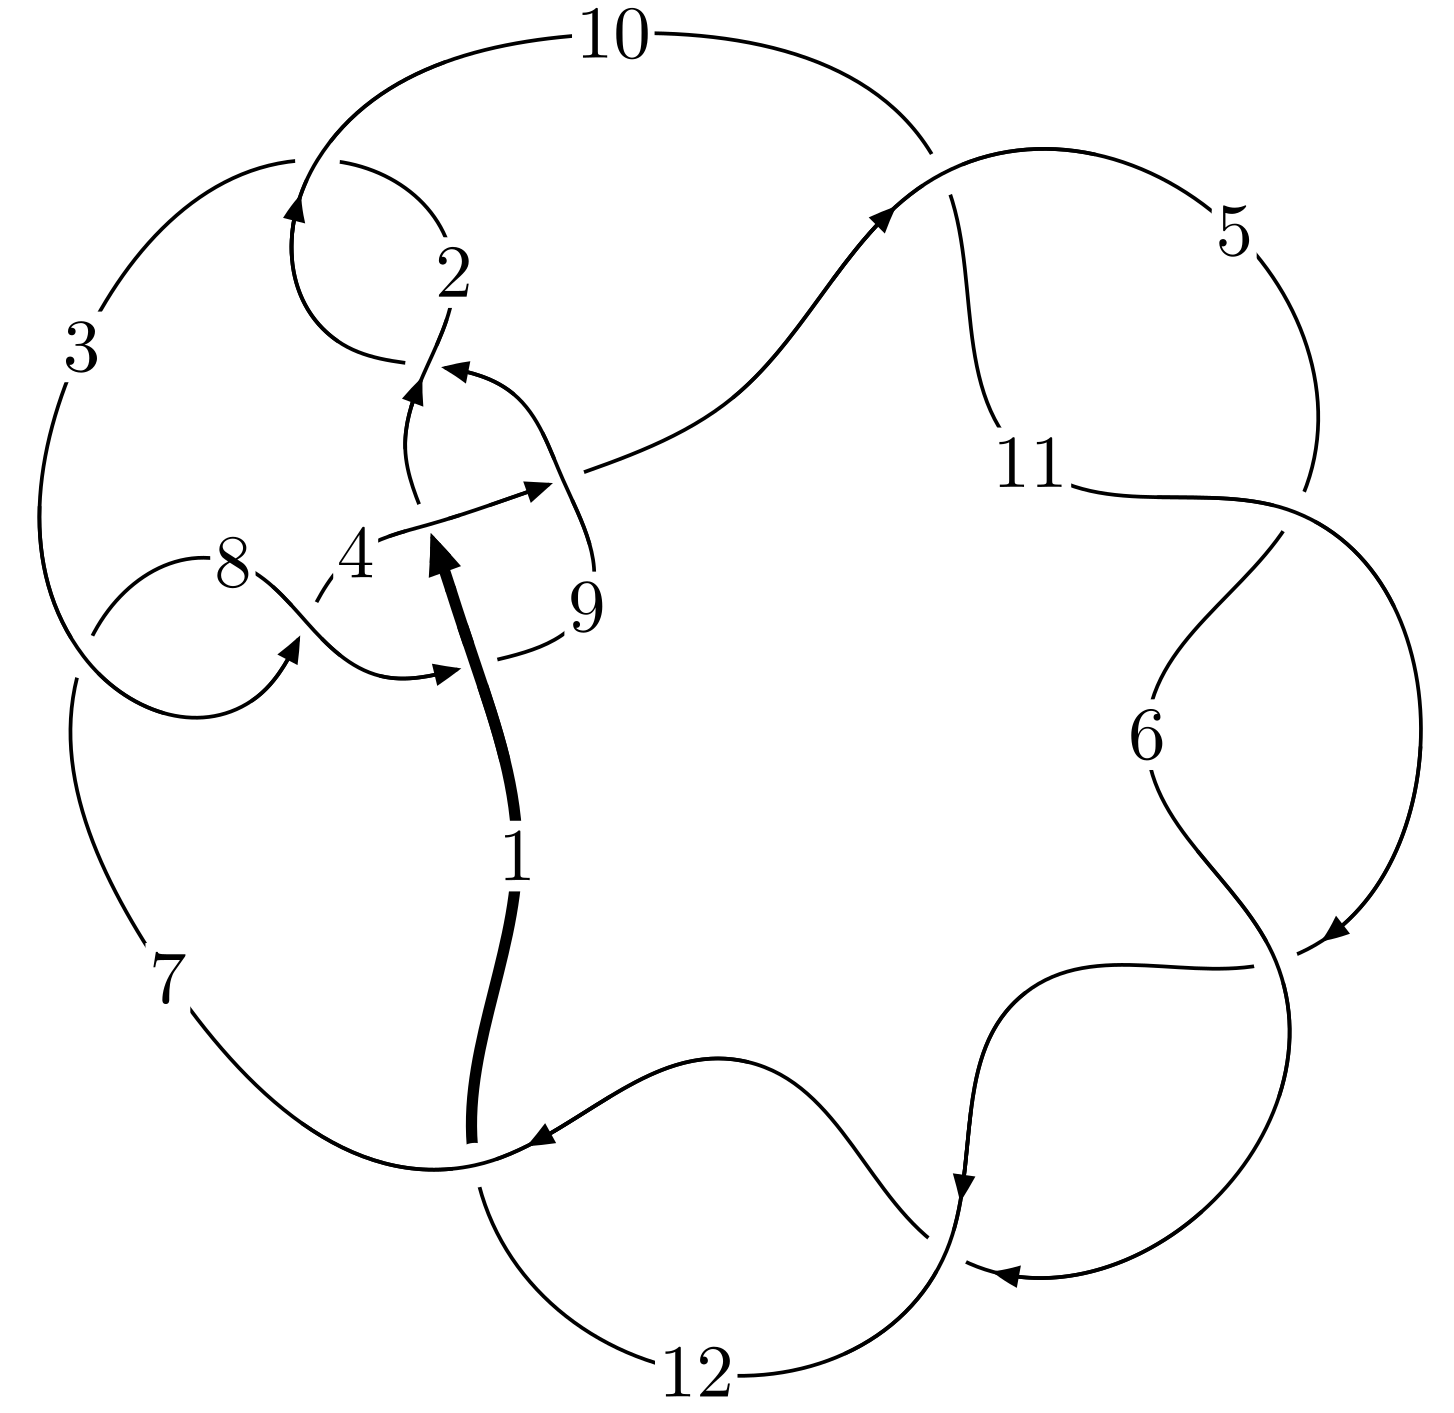
\includegraphics[width=112pt]{../../../GIT/diagram.site/Diagrams/png/1977_12a_1176.png}\\
\ \ \ A knot diagram\footnotemark}&
\allowdisplaybreaks
\textbf{Linearized knot diagam} \\
\cline{2-2}
 &
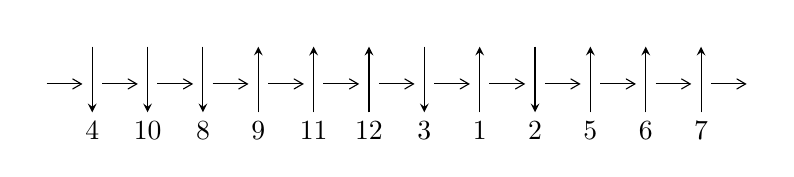
\begin{tikzpicture}[x=20pt, y=17pt]
	% nodes
	\node (C0) at (0, 0) {};
	\node (C1) at (1, 0) {};
	\node (C1U) at (1, +1) {};
	\node (C1D) at (1, -1) {4};

	\node (C2) at (2, 0) {};
	\node (C2U) at (2, +1) {};
	\node (C2D) at (2, -1) {10};

	\node (C3) at (3, 0) {};
	\node (C3U) at (3, +1) {};
	\node (C3D) at (3, -1) {8};

	\node (C4) at (4, 0) {};
	\node (C4U) at (4, +1) {};
	\node (C4D) at (4, -1) {9};

	\node (C5) at (5, 0) {};
	\node (C5U) at (5, +1) {};
	\node (C5D) at (5, -1) {11};

	\node (C6) at (6, 0) {};
	\node (C6U) at (6, +1) {};
	\node (C6D) at (6, -1) {12};

	\node (C7) at (7, 0) {};
	\node (C7U) at (7, +1) {};
	\node (C7D) at (7, -1) {3};

	\node (C8) at (8, 0) {};
	\node (C8U) at (8, +1) {};
	\node (C8D) at (8, -1) {1};

	\node (C9) at (9, 0) {};
	\node (C9U) at (9, +1) {};
	\node (C9D) at (9, -1) {2};

	\node (C10) at (10, 0) {};
	\node (C10U) at (10, +1) {};
	\node (C10D) at (10, -1) {5};

	\node (C11) at (11, 0) {};
	\node (C11U) at (11, +1) {};
	\node (C11D) at (11, -1) {6};

	\node (C12) at (12, 0) {};
	\node (C12U) at (12, +1) {};
	\node (C12D) at (12, -1) {7};
	\node (C13) at (13, 0) {};

	% arrows
	\draw[->,>={angle 60}]
	(C0) edge (C1) (C1) edge (C2) (C2) edge (C3) (C3) edge (C4) (C4) edge (C5) (C5) edge (C6) (C6) edge (C7) (C7) edge (C8) (C8) edge (C9) (C9) edge (C10) (C10) edge (C11) (C11) edge (C12) (C12) edge (C13) ;	\draw[->,>=stealth]
	(C1U) edge (C1D) (C2U) edge (C2D) (C3U) edge (C3D) (C4D) edge (C4U) (C5D) edge (C5U) (C6D) edge (C6U) (C7U) edge (C7D) (C8D) edge (C8U) (C9U) edge (C9D) (C10D) edge (C10U) (C11D) edge (C11U) (C12D) edge (C12U) ;
	\end{tikzpicture} \\
\hhline{~~} \\& 
\textbf{Solving Sequence} \\ \cline{2-2} 
 &
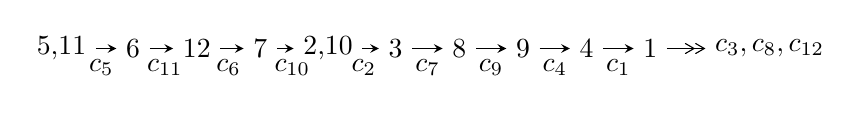
\begin{tikzpicture}[x=23pt, y=7pt]
	% node
	\node (A0) at (-1/8, 0) {5,11};
	\node (A1) at (1, 0) {6};
	\node (A2) at (2, 0) {12};
	\node (A3) at (3, 0) {7};
	\node (A4) at (65/16, 0) {2,10};
	\node (A5) at (41/8, 0) {3};
	\node (A6) at (49/8, 0) {8};
	\node (A7) at (57/8, 0) {9};
	\node (A8) at (65/8, 0) {4};
	\node (A9) at (73/8, 0) {1};
	\node (C1) at (1/2, -1) {$c_{5}$};
	\node (C2) at (3/2, -1) {$c_{11}$};
	\node (C3) at (5/2, -1) {$c_{6}$};
	\node (C4) at (7/2, -1) {$c_{10}$};
	\node (C5) at (37/8, -1) {$c_{2}$};
	\node (C6) at (45/8, -1) {$c_{7}$};
	\node (C7) at (53/8, -1) {$c_{9}$};
	\node (C8) at (61/8, -1) {$c_{4}$};
	\node (C9) at (69/8, -1) {$c_{1}$};
	\node (A10) at (11, 0) {$c_{3},c_{8},c_{12}$};

	% edge
	\draw[->,>=stealth]	
	(A0) edge (A1) (A1) edge (A2) (A2) edge (A3) (A3) edge (A4) (A4) edge (A5) (A5) edge (A6) (A6) edge (A7) (A7) edge (A8) (A8) edge (A9) ;
	\draw[->>,>={angle 60}]	
	(A9) edge (A10);
\end{tikzpicture} \\ 

\end{tabular} \\

\footnotetext{
The image of knot diagram is generated by the software ``\textbf{Draw programme}" developed by Andrew Bartholomew(\url{http://www.layer8.co.uk/maths/draw/index.htm\#Running-draw}), where we modified some parts for our purpose(\url{https://github.com/CATsTAILs/LinksPainter}).
}\phantom \\ \newline 
\centering \textbf{Ideals for irreducible components\footnotemark of $X_{\text{par}}$} 
 
\begin{align*}
I^u_{1}&=\langle 
-49 u^{23}+263 u^{22}+\cdots+4 b+236,\;273 u^{23}-1433 u^{22}+\cdots+8 a-1244,\;u^{24}-7 u^{23}+\cdots-32 u+8\rangle \\
I^u_{2}&=\langle 
-1.44275\times10^{19} a^{5} u^{7}-5.68398\times10^{19} a^{4} u^{7}+\cdots-3.60536\times10^{20} a+7.51047\times10^{20},\\
\phantom{I^u_{2}}&\phantom{= \langle  }6 u^7 a^4-4 u^7 a^3+\cdots-37 a-45,\;u^8+u^7-5 u^6-4 u^5+7 u^4+4 u^3-2 u^2-2 u-1\rangle \\
I^u_{3}&=\langle 
- u^8+6 u^6- u^5-11 u^4+3 u^3+6 u^2+b- u,\\
\phantom{I^u_{3}}&\phantom{= \langle  }- u^{12}- u^{11}+10 u^{10}+9 u^9-37 u^8-31 u^7+61 u^6+52 u^5-41 u^4-42 u^3+5 u^2+a+10 u+2,\\
\phantom{I^u_{3}}&\phantom{= \langle  }u^{13}-10 u^{11}+38 u^9+u^8-68 u^7-6 u^6+57 u^5+11 u^4-18 u^3-6 u^2+1\rangle \\
\\
\end{align*}
\raggedright * 3 irreducible components of $\dim_{\mathbb{C}}=0$, with total 85 representations.\\
\footnotetext{All coefficients of polynomials are rational numbers. But the coefficients are sometimes approximated in decimal forms when there is not enough margin.}
\newpage
\renewcommand{\arraystretch}{1}
\centering \section*{I. $I^u_{1}= \langle -49 u^{23}+263 u^{22}+\cdots+4 b+236,\;273 u^{23}-1433 u^{22}+\cdots+8 a-1244,\;u^{24}-7 u^{23}+\cdots-32 u+8 \rangle$}
\flushleft \textbf{(i) Arc colorings}\\
\begin{tabular}{m{7pt} m{180pt} m{7pt} m{180pt} }
\flushright $a_{5}=$&$\begin{pmatrix}1\\0\end{pmatrix}$ \\
\flushright $a_{11}=$&$\begin{pmatrix}0\\u\end{pmatrix}$ \\
\flushright $a_{6}=$&$\begin{pmatrix}1\\- u^2\end{pmatrix}$ \\
\flushright $a_{12}=$&$\begin{pmatrix}u\\- u^3+u\end{pmatrix}$ \\
\flushright $a_{7}=$&$\begin{pmatrix}- u^2+1\\u^4-2 u^2\end{pmatrix}$ \\
\flushright $a_{2}=$&$\begin{pmatrix}-\frac{273}{8} u^{23}+\frac{1433}{8} u^{22}+\cdots-532 u+\frac{311}{2}\\\frac{49}{4} u^{23}-\frac{263}{4} u^{22}+\cdots+\frac{403}{2} u-59\end{pmatrix}$ \\
\flushright $a_{10}=$&$\begin{pmatrix}- u\\u\end{pmatrix}$ \\
\flushright $a_{3}=$&$\begin{pmatrix}\frac{303}{8} u^{23}-\frac{1559}{8} u^{22}+\cdots+565 u-\frac{325}{2}\\-\frac{239}{4} u^{23}+\frac{1233}{4} u^{22}+\cdots-\frac{1791}{2} u+259\end{pmatrix}$ \\
\flushright $a_{8}=$&$\begin{pmatrix}26.2500 u^{23}-135.750 u^{22}+\cdots+395.500 u-113.500\\-\frac{79}{2} u^{23}+205 u^{22}+\cdots-\frac{1201}{2} u+174\end{pmatrix}$ \\
\flushright $a_{9}=$&$\begin{pmatrix}-15.2500 u^{23}+81.7500 u^{22}+\cdots-251.500 u+73.5000\\2 u^{23}-\frac{25}{2} u^{22}+\cdots+\frac{93}{2} u-14\end{pmatrix}$ \\
\flushright $a_{4}=$&$\begin{pmatrix}51 u^{23}-\frac{1075}{4} u^{22}+\cdots+\frac{3227}{4} u-235\\-\frac{129}{4} u^{23}+\frac{685}{4} u^{22}+\cdots-518 u+152\end{pmatrix}$ \\
\flushright $a_{1}=$&$\begin{pmatrix}- u^3+2 u\\u^5-3 u^3+u\end{pmatrix}$\\&\end{tabular}
\flushleft \textbf{(ii) Obstruction class $= -1$}\\~\\
\flushleft \textbf{(iii) Cusp Shapes $= 81 u^{23}-432 u^{22}+8 u^{21}+3419 u^{20}-3447 u^{19}-11374 u^{18}+17236 u^{17}+18946 u^{16}-40556 u^{15}-11583 u^{14}+53859 u^{13}-14035 u^{12}-38970 u^{11}+33571 u^{10}+7682 u^9-25123 u^8+11838 u^7+5007 u^6-9421 u^5+3205 u^4+124 u^3-1814 u^2+1300 u-374$}\\~\\
\newpage\renewcommand{\arraystretch}{1}
\flushleft \textbf{(iv) u-Polynomials at the component}\newline \\
\begin{tabular}{m{50pt}|m{274pt}}
Crossings & \hspace{64pt}u-Polynomials at each crossing \\
\hline $$\begin{aligned}c_{1}\end{aligned}$$&$\begin{aligned}
&u^{24}-18 u^{23}+\cdots+2816 u-256
\end{aligned}$\\
\hline $$\begin{aligned}c_{2},c_{3},c_{7}\\c_{9}\end{aligned}$$&$\begin{aligned}
&u^{24}- u^{23}+\cdots+u-1
\end{aligned}$\\
\hline $$\begin{aligned}c_{4},c_{8}\end{aligned}$$&$\begin{aligned}
&u^{24}-6 u^{22}+\cdots-2 u+1
\end{aligned}$\\
\hline $$\begin{aligned}c_{5},c_{6},c_{10}\\c_{11},c_{12}\end{aligned}$$&$\begin{aligned}
&u^{24}-7 u^{23}+\cdots-32 u+8
\end{aligned}$\\
\hline
\end{tabular}\\~\\
\newpage\renewcommand{\arraystretch}{1}
\flushleft \textbf{(v) Riley Polynomials at the component}\newline \\
\begin{tabular}{m{50pt}|m{274pt}}
Crossings & \hspace{64pt}Riley Polynomials at each crossing \\
\hline $$\begin{aligned}c_{1}\end{aligned}$$&$\begin{aligned}
&y^{24}-10 y^{23}+\cdots+262144 y+65536
\end{aligned}$\\
\hline $$\begin{aligned}c_{2},c_{3},c_{7}\\c_{9}\end{aligned}$$&$\begin{aligned}
&y^{24}-13 y^{23}+\cdots-3 y+1
\end{aligned}$\\
\hline $$\begin{aligned}c_{4},c_{8}\end{aligned}$$&$\begin{aligned}
&y^{24}-12 y^{23}+\cdots-30 y+1
\end{aligned}$\\
\hline $$\begin{aligned}c_{5},c_{6},c_{10}\\c_{11},c_{12}\end{aligned}$$&$\begin{aligned}
&y^{24}-31 y^{23}+\cdots-160 y+64
\end{aligned}$\\
\hline
\end{tabular}\\~\\
\newpage\flushleft \textbf{(vi) Complex Volumes and Cusp Shapes}
$$\begin{array}{c|c|c}  
\text{Solutions to }I^u_{1}& \I (\text{vol} + \sqrt{-1}CS) & \text{Cusp shape}\\
 \hline 
\begin{aligned}
u &= -0.907236 + 0.435980 I \\
a &= -1.41635 + 0.54146 I \\
b &= \phantom{-}0.86042 - 1.37712 I\end{aligned}
 & \phantom{-}1.84093 - 5.17326 I & \phantom{-}6.63681 + 8.84471 I \\ \hline\begin{aligned}
u &= -0.907236 - 0.435980 I \\
a &= -1.41635 - 0.54146 I \\
b &= \phantom{-}0.86042 + 1.37712 I\end{aligned}
 & \phantom{-}1.84093 + 5.17326 I & \phantom{-}6.63681 - 8.84471 I \\ \hline\begin{aligned}
u &= -1.110420 + 0.108192 I \\
a &= -0.180104 - 0.437950 I \\
b &= \phantom{-}0.385921 - 0.238265 I\end{aligned}
 & \phantom{-}5.73283 - 1.83988 I & \phantom{-}11.28356 + 2.30712 I \\ \hline\begin{aligned}
u &= -1.110420 - 0.108192 I \\
a &= -0.180104 + 0.437950 I \\
b &= \phantom{-}0.385921 + 0.238265 I\end{aligned}
 & \phantom{-}5.73283 + 1.83988 I & \phantom{-}11.28356 - 2.30712 I \\ \hline\begin{aligned}
u &= \phantom{-}0.590338 + 0.652762 I \\
a &= -1.171600 - 0.599827 I \\
b &= -0.006346 + 1.289090 I\end{aligned}
 & -4.24228 - 4.48435 I & -0.15247 + 3.55403 I \\ \hline\begin{aligned}
u &= \phantom{-}0.590338 - 0.652762 I \\
a &= -1.171600 + 0.599827 I \\
b &= -0.006346 - 1.289090 I\end{aligned}
 & -4.24228 + 4.48435 I & -0.15247 - 3.55403 I \\ \hline\begin{aligned}
u &= -1.048400 + 0.428308 I \\
a &= \phantom{-}1.79332 - 0.68716 I \\
b &= -0.92291 + 1.62751 I\end{aligned}
 & -1.26907 - 12.76890 I & \phantom{-}2.91843 + 8.75350 I \\ \hline\begin{aligned}
u &= -1.048400 - 0.428308 I \\
a &= \phantom{-}1.79332 + 0.68716 I \\
b &= -0.92291 - 1.62751 I\end{aligned}
 & -1.26907 + 12.76890 I & \phantom{-}2.91843 - 8.75350 I \\ \hline\begin{aligned}
u &= \phantom{-}0.242387 + 0.711300 I \\
a &= \phantom{-}0.388011 - 0.226722 I \\
b &= -0.46013 - 1.55775 I\end{aligned}
 & -5.25345 + 8.92776 I & -1.31883 - 7.64206 I \\ \hline\begin{aligned}
u &= \phantom{-}0.242387 - 0.711300 I \\
a &= \phantom{-}0.388011 + 0.226722 I \\
b &= -0.46013 + 1.55775 I\end{aligned}
 & -5.25345 - 8.92776 I & -1.31883 + 7.64206 I\\
 \hline 
 \end{array}$$\newpage$$\begin{array}{c|c|c}  
\text{Solutions to }I^u_{1}& \I (\text{vol} + \sqrt{-1}CS) & \text{Cusp shape}\\
 \hline 
\begin{aligned}
u &= \phantom{-}1.33594\phantom{ +0.000000I} \\
a &= \phantom{-}1.98547\phantom{ +0.000000I} \\
b &= -1.43379\phantom{ +0.000000I}\end{aligned}
 & \phantom{-}2.74446\phantom{ +0.000000I} & -2.28800\phantom{ +0.000000I} \\ \hline\begin{aligned}
u &= -0.016484 + 0.578692 I \\
a &= \phantom{-}0.554305 + 0.154675 I \\
b &= \phantom{-}0.093232 + 1.039400 I\end{aligned}
 & -0.87333 + 1.64838 I & \phantom{-}3.09303 - 4.00385 I \\ \hline\begin{aligned}
u &= -0.016484 - 0.578692 I \\
a &= \phantom{-}0.554305 - 0.154675 I \\
b &= \phantom{-}0.093232 - 1.039400 I\end{aligned}
 & -0.87333 - 1.64838 I & \phantom{-}3.09303 + 4.00385 I \\ \hline\begin{aligned}
u &= -1.43642 + 0.29668 I \\
a &= -1.124190 + 0.697341 I \\
b &= \phantom{-}0.437158 - 0.696629 I\end{aligned}
 & \phantom{-}2.30586 + 0.99863 I & \phantom{-}1.91156 - 3.99663 I \\ \hline\begin{aligned}
u &= -1.43642 - 0.29668 I \\
a &= -1.124190 - 0.697341 I \\
b &= \phantom{-}0.437158 + 0.696629 I\end{aligned}
 & \phantom{-}2.30586 - 0.99863 I & \phantom{-}1.91156 + 3.99663 I \\ \hline\begin{aligned}
u &= \phantom{-}0.417711 + 0.252673 I \\
a &= \phantom{-}0.709564 + 0.673149 I \\
b &= \phantom{-}0.223162 - 0.102887 I\end{aligned}
 & \phantom{-}0.898603 + 0.583790 I & \phantom{-}8.28194 - 3.24260 I \\ \hline\begin{aligned}
u &= \phantom{-}0.417711 - 0.252673 I \\
a &= \phantom{-}0.709564 - 0.673149 I \\
b &= \phantom{-}0.223162 + 0.102887 I\end{aligned}
 & \phantom{-}0.898603 - 0.583790 I & \phantom{-}8.28194 + 3.24260 I \\ \hline\begin{aligned}
u &= \phantom{-}1.69916 + 0.12248 I \\
a &= -1.96502 - 1.07970 I \\
b &= \phantom{-}1.40767 + 1.48523 I\end{aligned}
 & \phantom{-}10.97660 + 7.39354 I & \phantom{-}6.46638 - 6.79577 I \\ \hline\begin{aligned}
u &= \phantom{-}1.69916 - 0.12248 I \\
a &= -1.96502 + 1.07970 I \\
b &= \phantom{-}1.40767 - 1.48523 I\end{aligned}
 & \phantom{-}10.97660 - 7.39354 I & \phantom{-}6.46638 + 6.79577 I \\ \hline\begin{aligned}
u &= \phantom{-}1.73198 + 0.11712 I \\
a &= \phantom{-}2.05259 + 1.20136 I \\
b &= -1.29425 - 1.66429 I\end{aligned}
 & \phantom{-}8.5296 + 15.0189 I & \phantom{-0.000000 } 0. - 7.46096 I\\
 \hline 
 \end{array}$$\newpage$$\begin{array}{c|c|c}  
\text{Solutions to }I^u_{1}& \I (\text{vol} + \sqrt{-1}CS) & \text{Cusp shape}\\
 \hline 
\begin{aligned}
u &= \phantom{-}1.73198 - 0.11712 I \\
a &= \phantom{-}2.05259 - 1.20136 I \\
b &= -1.29425 + 1.66429 I\end{aligned}
 & \phantom{-}8.5296 - 15.0189 I & \phantom{-0.000000 -}0. + 7.46096 I \\ \hline\begin{aligned}
u &= \phantom{-}1.74907 + 0.02053 I \\
a &= -0.329253 - 0.013460 I \\
b &= \phantom{-}0.383663 + 0.561786 I\end{aligned}
 & \phantom{-}16.0549 + 2.3419 I & \phantom{-}10.98491 + 0. I\phantom{ +0.000000I} \\ \hline\begin{aligned}
u &= \phantom{-}1.74907 - 0.02053 I \\
a &= -0.329253 + 0.013460 I \\
b &= \phantom{-}0.383663 - 0.561786 I\end{aligned}
 & \phantom{-}16.0549 - 2.3419 I & \phantom{-}10.98491 + 0. I\phantom{ +0.000000I} \\ \hline\begin{aligned}
u &= \phantom{-}1.84069\phantom{ +0.000000I} \\
a &= -0.608035\phantom{ +0.000000I} \\
b &= \phantom{-}0.218649\phantom{ +0.000000I}\end{aligned}
 & \phantom{-}15.0349\phantom{ +0.000000I} & \phantom{-0.000000 } 0\\
 \hline 
 \end{array}$$\newpage\newpage\renewcommand{\arraystretch}{1}
\centering \section*{II. $I^u_{2}= \langle -1.44\times10^{19} a^{5} u^{7}-5.68\times10^{19} a^{4} u^{7}+\cdots-3.61\times10^{20} a+7.51\times10^{20},\;6 u^7 a^4-4 u^7 a^3+\cdots-37 a-45,\;u^8+u^7+\cdots-2 u-1 \rangle$}
\flushleft \textbf{(i) Arc colorings}\\
\begin{tabular}{m{7pt} m{180pt} m{7pt} m{180pt} }
\flushright $a_{5}=$&$\begin{pmatrix}1\\0\end{pmatrix}$ \\
\flushright $a_{11}=$&$\begin{pmatrix}0\\u\end{pmatrix}$ \\
\flushright $a_{6}=$&$\begin{pmatrix}1\\- u^2\end{pmatrix}$ \\
\flushright $a_{12}=$&$\begin{pmatrix}u\\- u^3+u\end{pmatrix}$ \\
\flushright $a_{7}=$&$\begin{pmatrix}- u^2+1\\u^4-2 u^2\end{pmatrix}$ \\
\flushright $a_{2}=$&$\begin{pmatrix}a\\0.0404307 a^{5} u^{7}+0.159284 a^{4} u^{7}+\cdots+1.01034 a-2.10469\end{pmatrix}$ \\
\flushright $a_{10}=$&$\begin{pmatrix}- u\\u\end{pmatrix}$ \\
\flushright $a_{3}=$&$\begin{pmatrix}-0.148451 a^{5} u^{7}+0.103349 a^{4} u^{7}+\cdots+0.884112 a+0.377445\\0.188881 a^{5} u^{7}+0.0559350 a^{4} u^{7}+\cdots+1.12623 a-2.48213\end{pmatrix}$ \\
\flushright $a_{8}=$&$\begin{pmatrix}0.0237472 a^{5} u^{7}-0.301682 a^{4} u^{7}+\cdots-1.09617 a+1.05392\\0.246102 a^{5} u^{7}-0.461154 a^{4} u^{7}+\cdots+0.187318 a+1.13432\end{pmatrix}$ \\
\flushright $a_{9}=$&$\begin{pmatrix}-0.0788423 a^{5} u^{7}+0.0602619 a^{4} u^{7}+\cdots-0.128977 a-1.90494\\0.0146164 a^{5} u^{7}+0.197157 a^{4} u^{7}+\cdots+1.71940 a-1.98699\end{pmatrix}$ \\
\flushright $a_{4}=$&$\begin{pmatrix}0.352334 a^{5} u^{7}-0.681823 a^{4} u^{7}+\cdots+0.871371 a+0.687129\\0.233033 a^{5} u^{7}-0.00868867 a^{4} u^{7}+\cdots+0.931401 a-2.76607\end{pmatrix}$ \\
\flushright $a_{1}=$&$\begin{pmatrix}- u^3+2 u\\u^5-3 u^3+u\end{pmatrix}$\\&\end{tabular}
\flushleft \textbf{(ii) Obstruction class $= -1$}\\~\\
\flushleft \textbf{(iii) Cusp Shapes $= \frac{20156225182067388064}{50977871582846282497} u^7 a^5+\frac{29676483013256697332}{50977871582846282497} u^7 a^4+\cdots+\frac{21731100052659838880}{50977871582846282497} a+\frac{182955131839228302618}{50977871582846282497}$}\\~\\
\newpage\renewcommand{\arraystretch}{1}
\flushleft \textbf{(iv) u-Polynomials at the component}\newline \\
\begin{tabular}{m{50pt}|m{274pt}}
Crossings & \hspace{64pt}u-Polynomials at each crossing \\
\hline $$\begin{aligned}c_{1}\end{aligned}$$&$\begin{aligned}
&(u^3+u^2-1)^{16}
\end{aligned}$\\
\hline $$\begin{aligned}c_{2},c_{3},c_{7}\\c_{9}\end{aligned}$$&$\begin{aligned}
&u^{48}+u^{47}+\cdots+628 u+199
\end{aligned}$\\
\hline $$\begin{aligned}c_{4},c_{8}\end{aligned}$$&$\begin{aligned}
&u^{48}+3 u^{47}+\cdots-34 u-1
\end{aligned}$\\
\hline $$\begin{aligned}c_{5},c_{6},c_{10}\\c_{11},c_{12}\end{aligned}$$&$\begin{aligned}
&(u^8+u^7-5 u^6-4 u^5+7 u^4+4 u^3-2 u^2-2 u-1)^6
\end{aligned}$\\
\hline
\end{tabular}\\~\\
\newpage\renewcommand{\arraystretch}{1}
\flushleft \textbf{(v) Riley Polynomials at the component}\newline \\
\begin{tabular}{m{50pt}|m{274pt}}
Crossings & \hspace{64pt}Riley Polynomials at each crossing \\
\hline $$\begin{aligned}c_{1}\end{aligned}$$&$\begin{aligned}
&(y^3- y^2+2 y-1)^{16}
\end{aligned}$\\
\hline $$\begin{aligned}c_{2},c_{3},c_{7}\\c_{9}\end{aligned}$$&$\begin{aligned}
&y^{48}-33 y^{47}+\cdots-434980 y+39601
\end{aligned}$\\
\hline $$\begin{aligned}c_{4},c_{8}\end{aligned}$$&$\begin{aligned}
&y^{48}+11 y^{47}+\cdots-668 y+1
\end{aligned}$\\
\hline $$\begin{aligned}c_{5},c_{6},c_{10}\\c_{11},c_{12}\end{aligned}$$&$\begin{aligned}
&(y^8-11 y^7+47 y^6-98 y^5+103 y^4-50 y^3+6 y^2+1)^6
\end{aligned}$\\
\hline
\end{tabular}\\~\\
\newpage\flushleft \textbf{(vi) Complex Volumes and Cusp Shapes}
$$\begin{array}{c|c|c}  
\text{Solutions to }I^u_{2}& \I (\text{vol} + \sqrt{-1}CS) & \text{Cusp shape}\\
 \hline 
\begin{aligned}
u &= \phantom{-}1.008780 + 0.254919 I \\
a &= -0.166634 - 0.860931 I \\
b &= -0.251079 - 0.246323 I\end{aligned}
 & \phantom{-}2.43453 + 6.46095 I & \phantom{-}5.93215 - 7.49747 I \\ \hline\begin{aligned}
u &= \phantom{-}1.008780 + 0.254919 I \\
a &= \phantom{-}0.980017 + 0.579991 I \\
b &= -0.240136 - 0.202961 I\end{aligned}
 & \phantom{-}2.43453 + 0.80471 I & \phantom{-}5.93215 - 1.53858 I \\ \hline\begin{aligned}
u &= \phantom{-}1.008780 + 0.254919 I \\
a &= \phantom{-}1.271630 + 0.216056 I \\
b &= -0.266125 - 1.193000 I\end{aligned}
 & -1.70306 + 3.63283 I & -0.59711 - 4.51802 I \\ \hline\begin{aligned}
u &= \phantom{-}1.008780 + 0.254919 I \\
a &= -0.68837 - 1.35983 I \\
b &= -0.25696 + 1.69313 I\end{aligned}
 & -1.70306 + 3.63283 I & -0.59711 - 4.51802 I \\ \hline\begin{aligned}
u &= \phantom{-}1.008780 + 0.254919 I \\
a &= \phantom{-}1.86379 + 0.32622 I \\
b &= -1.104540 - 0.808153 I\end{aligned}
 & \phantom{-}2.43453 + 0.80471 I & \phantom{-}5.93215 - 1.53858 I \\ \hline\begin{aligned}
u &= \phantom{-}1.008780 + 0.254919 I \\
a &= -2.23689 - 0.90869 I \\
b &= \phantom{-}1.20089 + 1.63498 I\end{aligned}
 & \phantom{-}2.43453 + 6.46095 I & \phantom{-}5.93215 - 7.49747 I \\ \hline\begin{aligned}
u &= \phantom{-}1.008780 - 0.254919 I \\
a &= -0.166634 + 0.860931 I \\
b &= -0.251079 + 0.246323 I\end{aligned}
 & \phantom{-}2.43453 - 6.46095 I & \phantom{-}5.93215 + 7.49747 I \\ \hline\begin{aligned}
u &= \phantom{-}1.008780 - 0.254919 I \\
a &= \phantom{-}0.980017 - 0.579991 I \\
b &= -0.240136 + 0.202961 I\end{aligned}
 & \phantom{-}2.43453 - 0.80471 I & \phantom{-}5.93215 + 1.53858 I \\ \hline\begin{aligned}
u &= \phantom{-}1.008780 - 0.254919 I \\
a &= \phantom{-}1.271630 - 0.216056 I \\
b &= -0.266125 + 1.193000 I\end{aligned}
 & -1.70306 - 3.63283 I & -0.59711 + 4.51802 I \\ \hline\begin{aligned}
u &= \phantom{-}1.008780 - 0.254919 I \\
a &= -0.68837 + 1.35983 I \\
b &= -0.25696 - 1.69313 I\end{aligned}
 & -1.70306 - 3.63283 I & -0.59711 + 4.51802 I\\
 \hline 
 \end{array}$$\newpage$$\begin{array}{c|c|c}  
\text{Solutions to }I^u_{2}& \I (\text{vol} + \sqrt{-1}CS) & \text{Cusp shape}\\
 \hline 
\begin{aligned}
u &= \phantom{-}1.008780 - 0.254919 I \\
a &= \phantom{-}1.86379 - 0.32622 I \\
b &= -1.104540 + 0.808153 I\end{aligned}
 & \phantom{-}2.43453 - 0.80471 I & \phantom{-}5.93215 + 1.53858 I \\ \hline\begin{aligned}
u &= \phantom{-}1.008780 - 0.254919 I \\
a &= -2.23689 + 0.90869 I \\
b &= \phantom{-}1.20089 - 1.63498 I\end{aligned}
 & \phantom{-}2.43453 - 6.46095 I & \phantom{-}5.93215 + 7.49747 I \\ \hline\begin{aligned}
u &= -0.772257\phantom{ +0.000000I} \\
a &= -1.364720 + 0.339718 I \\
b &= \phantom{-}0.223038 - 1.310810 I\end{aligned}
 & -0.55639 - 2.82812 I & \phantom{-}2.51294 + 2.97945 I \\ \hline\begin{aligned}
u &= -0.772257\phantom{ +0.000000I} \\
a &= -1.364720 - 0.339718 I \\
b &= \phantom{-}0.223038 + 1.310810 I\end{aligned}
 & -0.55639 + 2.82812 I & \phantom{-}2.51294 - 2.97945 I \\ \hline\begin{aligned}
u &= -0.772257\phantom{ +0.000000I} \\
a &= \phantom{-}1.70574 + 1.73282 I \\
b &= -0.72520 - 1.74104 I\end{aligned}
 & -0.55639 - 2.82812 I & \phantom{-}2.51294 + 2.97945 I \\ \hline\begin{aligned}
u &= -0.772257\phantom{ +0.000000I} \\
a &= \phantom{-}1.70574 - 1.73282 I \\
b &= -0.72520 + 1.74104 I\end{aligned}
 & -0.55639 + 2.82812 I & \phantom{-}2.51294 - 2.97945 I \\ \hline\begin{aligned}
u &= -0.772257\phantom{ +0.000000I} \\
a &= -2.61907\phantom{ +0.000000I} \\
b &= \phantom{-}0.283127\phantom{ +0.000000I}\end{aligned}
 & -4.69397\phantom{ +0.000000I} & -4.01630\phantom{ +0.000000I} \\ \hline\begin{aligned}
u &= -0.772257\phantom{ +0.000000I} \\
a &= \phantom{-}3.52258\phantom{ +0.000000I} \\
b &= -1.61356\phantom{ +0.000000I}\end{aligned}
 & -4.69397\phantom{ +0.000000I} & -4.01630\phantom{ +0.000000I} \\ \hline\begin{aligned}
u &= -0.240178 + 0.426557 I \\
a &= -0.900832 - 0.716113 I \\
b &= \phantom{-}0.49484 - 1.58079 I\end{aligned}
 & -1.41940 - 4.10344 I & \phantom{-}0.69028 + 8.06462 I \\ \hline\begin{aligned}
u &= -0.240178 + 0.426557 I \\
a &= -0.757692 - 0.900356 I \\
b &= -0.585477 - 1.229040 I\end{aligned}
 & -5.55698 - 1.27532 I & -5.83898 + 5.08518 I\\
 \hline 
 \end{array}$$\newpage$$\begin{array}{c|c|c}  
\text{Solutions to }I^u_{2}& \I (\text{vol} + \sqrt{-1}CS) & \text{Cusp shape}\\
 \hline 
\begin{aligned}
u &= -0.240178 + 0.426557 I \\
a &= \phantom{-}0.540126 - 0.065165 I \\
b &= -0.772436 + 0.638956 I\end{aligned}
 & -1.41940 + 1.55280 I & \phantom{-}0.69028 + 2.10573 I \\ \hline\begin{aligned}
u &= -0.240178 + 0.426557 I \\
a &= \phantom{-}1.70370 + 0.18215 I \\
b &= -0.068775 + 1.092420 I\end{aligned}
 & -1.41940 + 1.55280 I & \phantom{-}0.69028 + 2.10573 I \\ \hline\begin{aligned}
u &= -0.240178 + 0.426557 I \\
a &= -1.26218 + 1.32424 I \\
b &= -0.252731 - 0.328836 I\end{aligned}
 & -1.41940 - 4.10344 I & \phantom{-}0.69028 + 8.06462 I \\ \hline\begin{aligned}
u &= -0.240178 + 0.426557 I \\
a &= \phantom{-}0.86475 + 1.86092 I \\
b &= -0.208159 + 0.992906 I\end{aligned}
 & -5.55698 - 1.27532 I & -5.83898 + 5.08518 I \\ \hline\begin{aligned}
u &= -0.240178 - 0.426557 I \\
a &= -0.900832 + 0.716113 I \\
b &= \phantom{-}0.49484 + 1.58079 I\end{aligned}
 & -1.41940 + 4.10344 I & \phantom{-}0.69028 - 8.06462 I \\ \hline\begin{aligned}
u &= -0.240178 - 0.426557 I \\
a &= -0.757692 + 0.900356 I \\
b &= -0.585477 + 1.229040 I\end{aligned}
 & -5.55698 + 1.27532 I & -5.83898 - 5.08518 I \\ \hline\begin{aligned}
u &= -0.240178 - 0.426557 I \\
a &= \phantom{-}0.540126 + 0.065165 I \\
b &= -0.772436 - 0.638956 I\end{aligned}
 & -1.41940 - 1.55280 I & \phantom{-}0.69028 - 2.10573 I \\ \hline\begin{aligned}
u &= -0.240178 - 0.426557 I \\
a &= \phantom{-}1.70370 - 0.18215 I \\
b &= -0.068775 - 1.092420 I\end{aligned}
 & -1.41940 - 1.55280 I & \phantom{-}0.69028 - 2.10573 I \\ \hline\begin{aligned}
u &= -0.240178 - 0.426557 I \\
a &= -1.26218 - 1.32424 I \\
b &= -0.252731 + 0.328836 I\end{aligned}
 & -1.41940 + 4.10344 I & \phantom{-}0.69028 - 8.06462 I \\ \hline\begin{aligned}
u &= -0.240178 - 0.426557 I \\
a &= \phantom{-}0.86475 - 1.86092 I \\
b &= -0.208159 - 0.992906 I\end{aligned}
 & -5.55698 + 1.27532 I & -5.83898 - 5.08518 I\\
 \hline 
 \end{array}$$\newpage$$\begin{array}{c|c|c}  
\text{Solutions to }I^u_{2}& \I (\text{vol} + \sqrt{-1}CS) & \text{Cusp shape}\\
 \hline 
\begin{aligned}
u &= \phantom{-}1.67992\phantom{ +0.000000I} \\
a &= -1.22399 + 0.97102 I \\
b &= \phantom{-}0.58572 - 1.53466 I\end{aligned}
 & \phantom{-}8.26521 - 2.82812 I & \phantom{-}3.33185 + 2.97945 I \\ \hline\begin{aligned}
u &= \phantom{-}1.67992\phantom{ +0.000000I} \\
a &= -1.22399 - 0.97102 I \\
b &= \phantom{-}0.58572 + 1.53466 I\end{aligned}
 & \phantom{-}8.26521 + 2.82812 I & \phantom{-}3.33185 - 2.97945 I \\ \hline\begin{aligned}
u &= \phantom{-}1.67992\phantom{ +0.000000I} \\
a &= -2.06031\phantom{ +0.000000I} \\
b &= \phantom{-}0.835472\phantom{ +0.000000I}\end{aligned}
 & \phantom{-}4.12763\phantom{ +0.000000I} & -3.19740\phantom{ +0.000000I} \\ \hline\begin{aligned}
u &= \phantom{-}1.67992\phantom{ +0.000000I} \\
a &= \phantom{-}1.71698 + 2.02515 I \\
b &= -1.19582 - 2.17322 I\end{aligned}
 & \phantom{-}8.26521 - 2.82812 I & \phantom{-}3.33185 + 2.97945 I \\ \hline\begin{aligned}
u &= \phantom{-}1.67992\phantom{ +0.000000I} \\
a &= \phantom{-}1.71698 - 2.02515 I \\
b &= -1.19582 + 2.17322 I\end{aligned}
 & \phantom{-}8.26521 + 2.82812 I & \phantom{-}3.33185 - 2.97945 I \\ \hline\begin{aligned}
u &= \phantom{-}1.67992\phantom{ +0.000000I} \\
a &= \phantom{-}3.36647\phantom{ +0.000000I} \\
b &= -2.45190\phantom{ +0.000000I}\end{aligned}
 & \phantom{-}4.12763\phantom{ +0.000000I} & -3.19740\phantom{ +0.000000I} \\ \hline\begin{aligned}
u &= -1.72243 + 0.06628 I \\
a &= \phantom{-}1.108900 - 0.735799 I \\
b &= -0.423485 + 1.321650 I\end{aligned}
 & \phantom{-}8.02419 - 4.93524 I & -0.03508 + 2.99422 I \\ \hline\begin{aligned}
u &= -1.72243 + 0.06628 I \\
a &= \phantom{-}0.564850 - 0.069165 I \\
b &= -0.193774 - 0.376350 I\end{aligned}
 & \phantom{-}12.16180 - 2.10712 I & \phantom{-}6.49419 + 0.01478 I \\ \hline\begin{aligned}
u &= -1.72243 + 0.06628 I \\
a &= \phantom{-}0.091340 + 0.181993 I \\
b &= -0.257409 + 0.636530 I\end{aligned}
 & \phantom{-}12.1618 - 7.7634 I & \phantom{-}6.49419 + 5.97367 I \\ \hline\begin{aligned}
u &= -1.72243 + 0.06628 I \\
a &= -0.62469 + 1.84935 I \\
b &= \phantom{-}0.07951 - 2.00864 I\end{aligned}
 & \phantom{-}8.02419 - 4.93524 I & -0.03508 + 2.99422 I\\
 \hline 
 \end{array}$$\newpage$$\begin{array}{c|c|c}  
\text{Solutions to }I^u_{2}& \I (\text{vol} + \sqrt{-1}CS) & \text{Cusp shape}\\
 \hline 
\begin{aligned}
u &= -1.72243 + 0.06628 I \\
a &= \phantom{-}2.17225 - 0.62127 I \\
b &= -1.51193 + 0.90608 I\end{aligned}
 & \phantom{-}12.16180 - 2.10712 I & \phantom{-}6.49419 + 0.01478 I \\ \hline\begin{aligned}
u &= -1.72243 + 0.06628 I \\
a &= -2.46292 + 1.34903 I \\
b &= \phantom{-}1.70346 - 1.68486 I\end{aligned}
 & \phantom{-}12.1618 - 7.7634 I & \phantom{-}6.49419 + 5.97367 I \\ \hline\begin{aligned}
u &= -1.72243 - 0.06628 I \\
a &= \phantom{-}1.108900 + 0.735799 I \\
b &= -0.423485 - 1.321650 I\end{aligned}
 & \phantom{-}8.02419 + 4.93524 I & -0.03508 - 2.99422 I \\ \hline\begin{aligned}
u &= -1.72243 - 0.06628 I \\
a &= \phantom{-}0.564850 + 0.069165 I \\
b &= -0.193774 + 0.376350 I\end{aligned}
 & \phantom{-}12.16180 + 2.10712 I & \phantom{-}6.49419 - 0.01478 I \\ \hline\begin{aligned}
u &= -1.72243 - 0.06628 I \\
a &= \phantom{-}0.091340 - 0.181993 I \\
b &= -0.257409 - 0.636530 I\end{aligned}
 & \phantom{-}12.1618 + 7.7634 I & \phantom{-}6.49419 - 5.97367 I \\ \hline\begin{aligned}
u &= -1.72243 - 0.06628 I \\
a &= -0.62469 - 1.84935 I \\
b &= \phantom{-}0.07951 + 2.00864 I\end{aligned}
 & \phantom{-}8.02419 + 4.93524 I & -0.03508 - 2.99422 I \\ \hline\begin{aligned}
u &= -1.72243 - 0.06628 I \\
a &= \phantom{-}2.17225 + 0.62127 I \\
b &= -1.51193 - 0.90608 I\end{aligned}
 & \phantom{-}12.16180 + 2.10712 I & \phantom{-}6.49419 - 0.01478 I \\ \hline\begin{aligned}
u &= -1.72243 - 0.06628 I \\
a &= -2.46292 - 1.34903 I \\
b &= \phantom{-}1.70346 + 1.68486 I\end{aligned}
 & \phantom{-}12.1618 + 7.7634 I & \phantom{-}6.49419 - 5.97367 I\\
 \hline 
 \end{array}$$\newpage\newpage\renewcommand{\arraystretch}{1}
\centering \section*{III. $I^u_{3}= \langle - u^8+6 u^6- u^5-11 u^4+3 u^3+6 u^2+b- u,\;- u^{12}- u^{11}+\cdots+a+2,\;u^{13}-10 u^{11}+\cdots-6 u^2+1 \rangle$}
\flushleft \textbf{(i) Arc colorings}\\
\begin{tabular}{m{7pt} m{180pt} m{7pt} m{180pt} }
\flushright $a_{5}=$&$\begin{pmatrix}1\\0\end{pmatrix}$ \\
\flushright $a_{11}=$&$\begin{pmatrix}0\\u\end{pmatrix}$ \\
\flushright $a_{6}=$&$\begin{pmatrix}1\\- u^2\end{pmatrix}$ \\
\flushright $a_{12}=$&$\begin{pmatrix}u\\- u^3+u\end{pmatrix}$ \\
\flushright $a_{7}=$&$\begin{pmatrix}- u^2+1\\u^4-2 u^2\end{pmatrix}$ \\
\flushright $a_{2}=$&$\begin{pmatrix}u^{12}+u^{11}+\cdots-10 u-2\\u^8-6 u^6+u^5+11 u^4-3 u^3-6 u^2+u\end{pmatrix}$ \\
\flushright $a_{10}=$&$\begin{pmatrix}- u\\u\end{pmatrix}$ \\
\flushright $a_{3}=$&$\begin{pmatrix}u^{12}-10 u^{10}+\cdots-9 u-1\\u^{11}-8 u^9+u^8+23 u^7-5 u^6-28 u^5+7 u^4+12 u^3-2 u^2-1\end{pmatrix}$ \\
\flushright $a_{8}=$&$\begin{pmatrix}u^{10}+u^9-8 u^8-7 u^7+23 u^6+18 u^5-27 u^4-21 u^3+8 u^2+10 u+3\\- u^{12}+9 u^{10}- u^9-30 u^8+5 u^7+45 u^6-6 u^5-29 u^4- u^3+6 u^2+2 u\end{pmatrix}$ \\
\flushright $a_{9}=$&$\begin{pmatrix}u^{10}-8 u^8- u^7+23 u^6+7 u^5-28 u^4-15 u^3+11 u^2+10 u+2\\- u^{12}+9 u^{10}-30 u^8- u^7+45 u^6+5 u^5-29 u^4-7 u^3+6 u^2+2 u\end{pmatrix}$ \\
\flushright $a_{4}=$&$\begin{pmatrix}- u^{12}- u^{11}+\cdots+7 u+5\\- u^3+2 u\end{pmatrix}$ \\
\flushright $a_{1}=$&$\begin{pmatrix}- u^3+2 u\\u^5-3 u^3+u\end{pmatrix}$\\&\end{tabular}
\flushleft \textbf{(ii) Obstruction class $= 1$}\\~\\
\flushleft \textbf{(iii) Cusp Shapes $= 4 u^{12}-38 u^{10}+131 u^8+3 u^7-193 u^6-21 u^5+101 u^4+40 u^3+8 u^2-13 u-8$}\\~\\
\newpage\renewcommand{\arraystretch}{1}
\flushleft \textbf{(iv) u-Polynomials at the component}\newline \\
\begin{tabular}{m{50pt}|m{274pt}}
Crossings & \hspace{64pt}u-Polynomials at each crossing \\
\hline $$\begin{aligned}c_{1}\end{aligned}$$&$\begin{aligned}
&u^{13}-5 u^{12}+\cdots+4 u^2-1
\end{aligned}$\\
\hline $$\begin{aligned}c_{2},c_{7}\end{aligned}$$&$\begin{aligned}
&u^{13}+u^{12}+\cdots+u+1
\end{aligned}$\\
\hline $$\begin{aligned}c_{3},c_{9}\end{aligned}$$&$\begin{aligned}
&u^{13}- u^{12}+\cdots+u-1
\end{aligned}$\\
\hline $$\begin{aligned}c_{4},c_{8}\end{aligned}$$&$\begin{aligned}
&u^{13}+u^{10}-4 u^9+u^8- u^7+3 u^5-2 u^4+u^3-2 u^2+1
\end{aligned}$\\
\hline $$\begin{aligned}c_{5},c_{6}\end{aligned}$$&$\begin{aligned}
&u^{13}-10 u^{11}+38 u^9+u^8-68 u^7-6 u^6+57 u^5+11 u^4-18 u^3-6 u^2+1
\end{aligned}$\\
\hline $$\begin{aligned}c_{10},c_{11},c_{12}\end{aligned}$$&$\begin{aligned}
&u^{13}-10 u^{11}+38 u^9- u^8-68 u^7+6 u^6+57 u^5-11 u^4-18 u^3+6 u^2-1
\end{aligned}$\\
\hline
\end{tabular}\\~\\
\newpage\renewcommand{\arraystretch}{1}
\flushleft \textbf{(v) Riley Polynomials at the component}\newline \\
\begin{tabular}{m{50pt}|m{274pt}}
Crossings & \hspace{64pt}Riley Polynomials at each crossing \\
\hline $$\begin{aligned}c_{1}\end{aligned}$$&$\begin{aligned}
&y^{13}-9 y^{12}+\cdots+8 y-1
\end{aligned}$\\
\hline $$\begin{aligned}c_{2},c_{3},c_{7}\\c_{9}\end{aligned}$$&$\begin{aligned}
&y^{13}-13 y^{12}+\cdots+13 y-1
\end{aligned}$\\
\hline $$\begin{aligned}c_{4},c_{8}\end{aligned}$$&$\begin{aligned}
&y^{13}-8 y^{11}-3 y^{10}+20 y^9+9 y^8-19 y^7-6 y^6+9 y^5-7 y^3+4 y-1
\end{aligned}$\\
\hline $$\begin{aligned}c_{5},c_{6},c_{10}\\c_{11},c_{12}\end{aligned}$$&$\begin{aligned}
&y^{13}-20 y^{12}+\cdots+12 y-1
\end{aligned}$\\
\hline
\end{tabular}\\~\\
\newpage\flushleft \textbf{(vi) Complex Volumes and Cusp Shapes}
$$\begin{array}{c|c|c}  
\text{Solutions to }I^u_{3}& \I (\text{vol} + \sqrt{-1}CS) & \text{Cusp shape}\\
 \hline 
\begin{aligned}
u &= -0.900642 + 0.211290 I \\
a &= -0.806576 + 0.876637 I \\
b &= \phantom{-}0.07621 - 1.64069 I\end{aligned}
 & \phantom{-}0.15794 - 4.22361 I & \phantom{-}4.67376 + 7.74732 I \\ \hline\begin{aligned}
u &= -0.900642 - 0.211290 I \\
a &= -0.806576 - 0.876637 I \\
b &= \phantom{-}0.07621 + 1.64069 I\end{aligned}
 & \phantom{-}0.15794 + 4.22361 I & \phantom{-}4.67376 - 7.74732 I \\ \hline\begin{aligned}
u &= \phantom{-}0.835287\phantom{ +0.000000I} \\
a &= \phantom{-}3.11335\phantom{ +0.000000I} \\
b &= -1.13883\phantom{ +0.000000I}\end{aligned}
 & -4.06419\phantom{ +0.000000I} & \phantom{-}11.1840\phantom{ +0.000000I} \\ \hline\begin{aligned}
u &= \phantom{-}1.349780 + 0.188354 I \\
a &= \phantom{-}1.53326 + 0.73818 I \\
b &= -1.030280 - 0.706563 I\end{aligned}
 & \phantom{-}3.33191 - 0.41146 I & \phantom{-}8.75330 + 4.03305 I \\ \hline\begin{aligned}
u &= \phantom{-}1.349780 - 0.188354 I \\
a &= \phantom{-}1.53326 - 0.73818 I \\
b &= -1.030280 + 0.706563 I\end{aligned}
 & \phantom{-}3.33191 + 0.41146 I & \phantom{-}8.75330 - 4.03305 I \\ \hline\begin{aligned}
u &= -1.48165\phantom{ +0.000000I} \\
a &= -1.60389\phantom{ +0.000000I} \\
b &= \phantom{-}0.723464\phantom{ +0.000000I}\end{aligned}
 & \phantom{-}0.435715\phantom{ +0.000000I} & -0.725220\phantom{ +0.000000I} \\ \hline\begin{aligned}
u &= -0.246497 + 0.330591 I \\
a &= \phantom{-}2.16431 - 0.42060 I \\
b &= -0.44057 + 1.37835 I\end{aligned}
 & -2.02748 + 2.39614 I & -5.69138 - 3.50014 I \\ \hline\begin{aligned}
u &= -0.246497 - 0.330591 I \\
a &= \phantom{-}2.16431 + 0.42060 I \\
b &= -0.44057 - 1.37835 I\end{aligned}
 & -2.02748 - 2.39614 I & -5.69138 + 3.50014 I \\ \hline\begin{aligned}
u &= \phantom{-}0.333287\phantom{ +0.000000I} \\
a &= -4.10575\phantom{ +0.000000I} \\
b &= -0.312491\phantom{ +0.000000I}\end{aligned}
 & -5.76311\phantom{ +0.000000I} & -9.04720\phantom{ +0.000000I} \\ \hline\begin{aligned}
u &= -1.68760\phantom{ +0.000000I} \\
a &= \phantom{-}2.68033\phantom{ +0.000000I} \\
b &= -1.63543\phantom{ +0.000000I}\end{aligned}
 & \phantom{-}4.96623\phantom{ +0.000000I} & \phantom{-}8.76410\phantom{ +0.000000I}\\
 \hline 
 \end{array}$$\newpage$$\begin{array}{c|c|c}  
\text{Solutions to }I^u_{3}& \I (\text{vol} + \sqrt{-1}CS) & \text{Cusp shape}\\
 \hline 
\begin{aligned}
u &= \phantom{-}1.70777 + 0.05845 I \\
a &= -0.84719 - 1.38187 I \\
b &= \phantom{-}0.35559 + 1.80257 I\end{aligned}
 & \phantom{-}9.50181 + 5.30924 I & \phantom{-}6.33383 - 5.02700 I \\ \hline\begin{aligned}
u &= \phantom{-}1.70777 - 0.05845 I \\
a &= -0.84719 + 1.38187 I \\
b &= \phantom{-}0.35559 - 1.80257 I\end{aligned}
 & \phantom{-}9.50181 - 5.30924 I & \phantom{-}6.33383 + 5.02700 I \\ \hline\begin{aligned}
u &= -1.82016\phantom{ +0.000000I} \\
a &= \phantom{-}0.828351\phantom{ +0.000000I} \\
b &= -0.558619\phantom{ +0.000000I}\end{aligned}
 & \phantom{-}15.3957\phantom{ +0.000000I} & \phantom{-}16.6850\phantom{ +0.000000I}\\
 \hline 
 \end{array}$$\newpage
\newpage\renewcommand{\arraystretch}{1}
\centering \section*{ IV. u-Polynomials}
\begin{tabular}{m{50pt}|m{274pt}}
Crossings & \hspace{64pt}u-Polynomials at each crossing \\
\hline $$\begin{aligned}c_{1}\end{aligned}$$&$\begin{aligned}
&((u^3+u^2-1)^{16})(u^{13}-5 u^{12}+\cdots+4 u^2-1)\\
&\cdot(u^{24}-18 u^{23}+\cdots+2816 u-256)
\end{aligned}$\\
\hline $$\begin{aligned}c_{2},c_{7}\end{aligned}$$&$\begin{aligned}
&(u^{13}+u^{12}+\cdots+u+1)(u^{24}- u^{23}+\cdots+u-1)\\
&\cdot(u^{48}+u^{47}+\cdots+628 u+199)
\end{aligned}$\\
\hline $$\begin{aligned}c_{3},c_{9}\end{aligned}$$&$\begin{aligned}
&(u^{13}- u^{12}+\cdots+u-1)(u^{24}- u^{23}+\cdots+u-1)\\
&\cdot(u^{48}+u^{47}+\cdots+628 u+199)
\end{aligned}$\\
\hline $$\begin{aligned}c_{4},c_{8}\end{aligned}$$&$\begin{aligned}
&(u^{13}+u^{10}-4 u^9+u^8- u^7+3 u^5-2 u^4+u^3-2 u^2+1)\\
&\cdot(u^{24}-6 u^{22}+\cdots-2 u+1)(u^{48}+3 u^{47}+\cdots-34 u-1)
\end{aligned}$\\
\hline $$\begin{aligned}c_{5},c_{6}\end{aligned}$$&$\begin{aligned}
&(u^8+u^7-5 u^6-4 u^5+7 u^4+4 u^3-2 u^2-2 u-1)^6\\
&\cdot(u^{13}-10 u^{11}+38 u^9+u^8-68 u^7-6 u^6+57 u^5+11 u^4-18 u^3-6 u^2+1)\\
&\cdot(u^{24}-7 u^{23}+\cdots-32 u+8)
\end{aligned}$\\
\hline $$\begin{aligned}c_{10},c_{11},c_{12}\end{aligned}$$&$\begin{aligned}
&(u^8+u^7-5 u^6-4 u^5+7 u^4+4 u^3-2 u^2-2 u-1)^6\\
&\cdot(u^{13}-10 u^{11}+38 u^9- u^8-68 u^7+6 u^6+57 u^5-11 u^4-18 u^3+6 u^2-1)\\
&\cdot(u^{24}-7 u^{23}+\cdots-32 u+8)
\end{aligned}$\\
\hline
\end{tabular}\newpage\renewcommand{\arraystretch}{1}
\centering \section*{ V. Riley Polynomials}
\begin{tabular}{m{50pt}|m{274pt}}
Crossings & \hspace{64pt}Riley Polynomials at each crossing \\
\hline $$\begin{aligned}c_{1}\end{aligned}$$&$\begin{aligned}
&((y^3- y^2+2 y-1)^{16})(y^{13}-9 y^{12}+\cdots+8 y-1)\\
&\cdot(y^{24}-10 y^{23}+\cdots+262144 y+65536)
\end{aligned}$\\
\hline $$\begin{aligned}c_{2},c_{3},c_{7}\\c_{9}\end{aligned}$$&$\begin{aligned}
&(y^{13}-13 y^{12}+\cdots+13 y-1)(y^{24}-13 y^{23}+\cdots-3 y+1)\\
&\cdot(y^{48}-33 y^{47}+\cdots-434980 y+39601)
\end{aligned}$\\
\hline $$\begin{aligned}c_{4},c_{8}\end{aligned}$$&$\begin{aligned}
&(y^{13}-8 y^{11}-3 y^{10}+20 y^9+9 y^8-19 y^7-6 y^6+9 y^5-7 y^3+4 y-1)\\
&\cdot(y^{24}-12 y^{23}+\cdots-30 y+1)(y^{48}+11 y^{47}+\cdots-668 y+1)
\end{aligned}$\\
\hline $$\begin{aligned}c_{5},c_{6},c_{10}\\c_{11},c_{12}\end{aligned}$$&$\begin{aligned}
&(y^8-11 y^7+47 y^6-98 y^5+103 y^4-50 y^3+6 y^2+1)^6\\
&\cdot(y^{13}-20 y^{12}+\cdots+12 y-1)(y^{24}-31 y^{23}+\cdots-160 y+64)
\end{aligned}$\\
\hline
\end{tabular}
\vskip 2pc
\end{document}